\chapter{System Design}

\section{System / Software Design}

The system architecture is engineered as an offline experimental pipeline separating data ingestion, classifier inference, multi-signal extraction, review queue triage, and feedback adaptation.

\subsection{11.1 Architecture Diagram}

Figure 11.1 illustrates the high-level system architecture, showing the end-to-end dataflow from raw network telemetry to the prioritized human review queue and simulated feedback loop.

\begin{figure}[H]
\centering
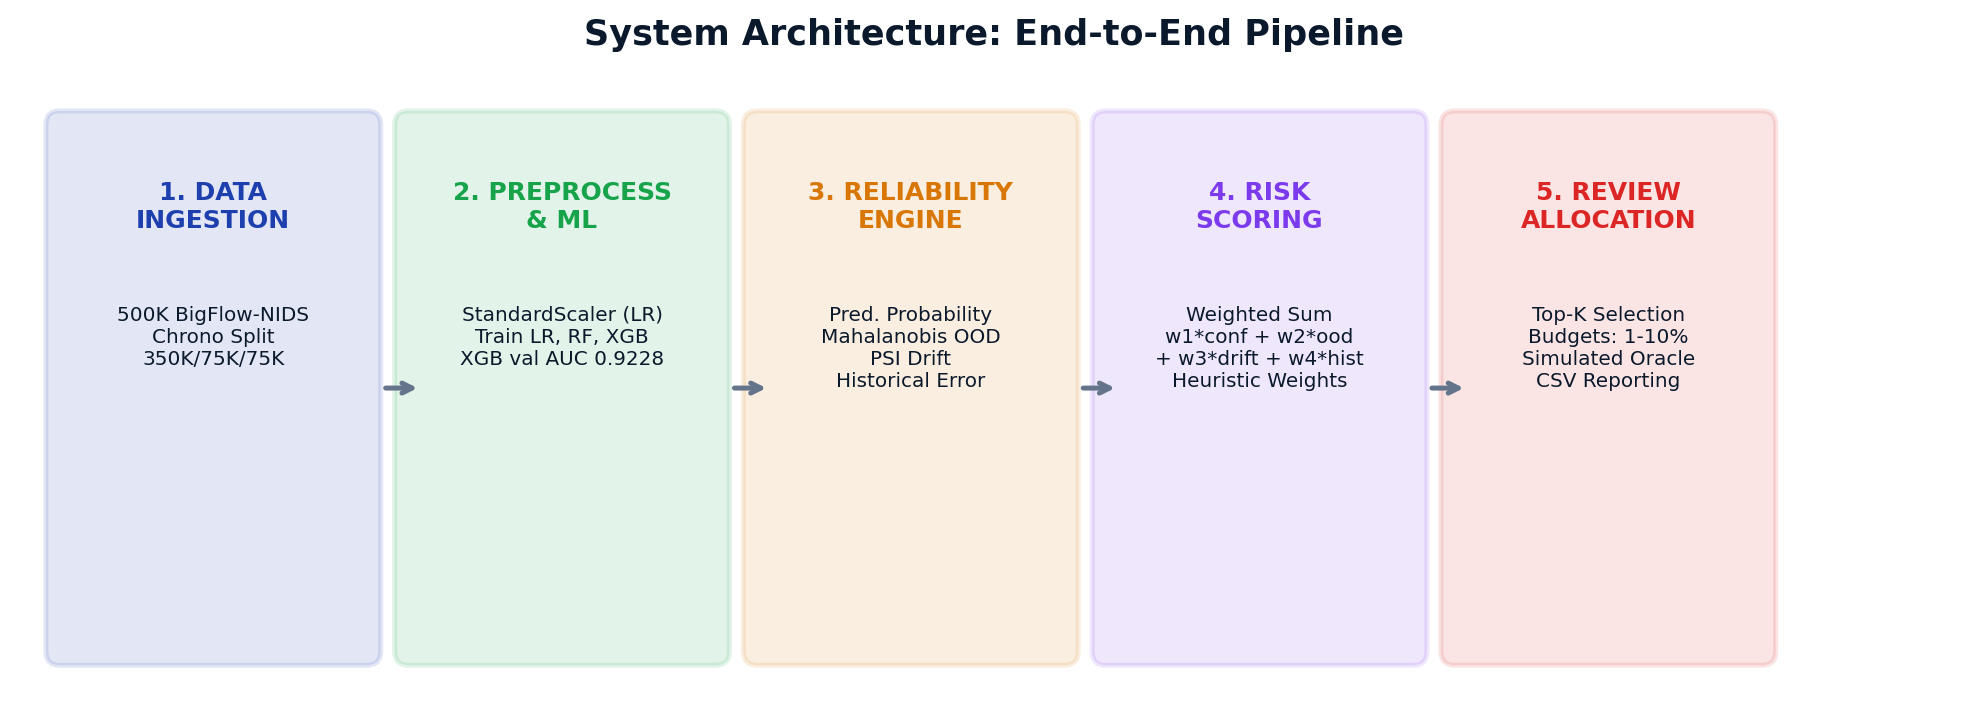
\includegraphics[width=0.85\textwidth]{figures/v2_architecture.png}
\caption{Figure 11.1: End-to-End System Architecture for Adaptive Human-Review Allocation.}
\end{figure}

\subsection{11.2 Use-Case Diagram}

Figure 11.2 presents the UML Use-Case Diagram depicting interactions between the primary actors (ML Practitioner, Security Analyst Reviewer, and System Evaluator) and system functional modules.

\begin{figure}[H]
\centering
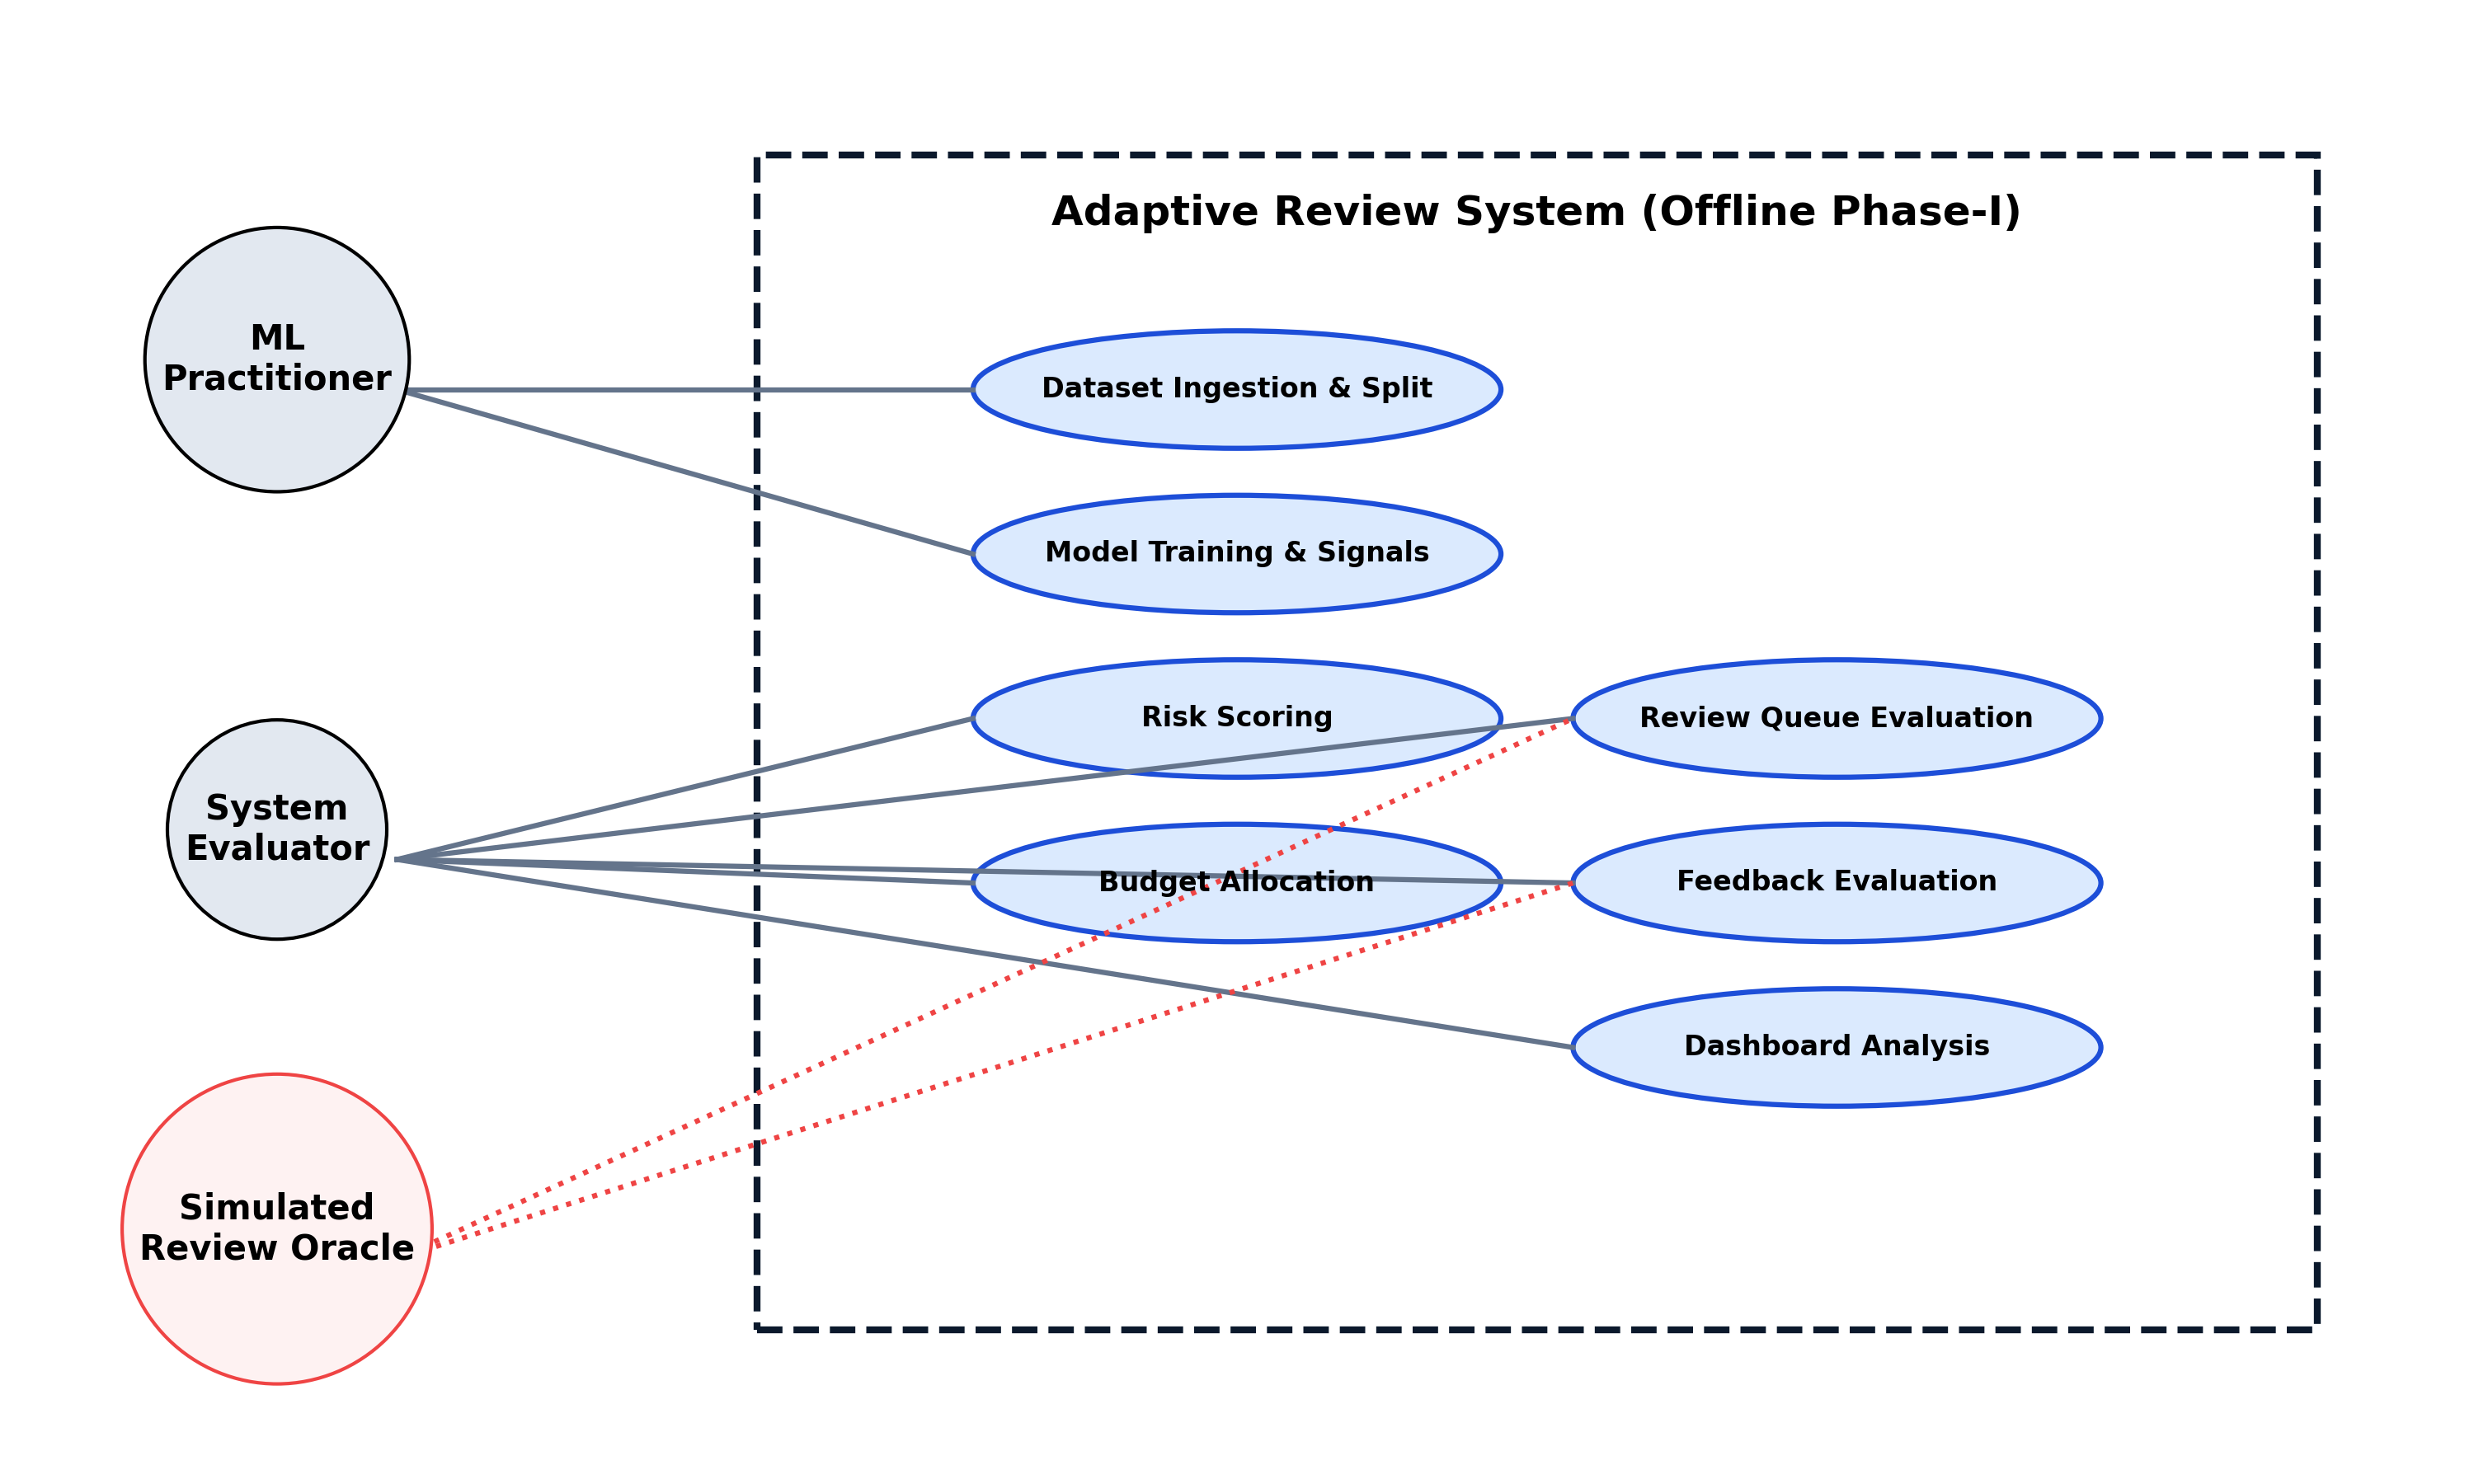
\includegraphics[width=0.85\textwidth]{figures/v2_use_case.png}
\caption{Figure 11.2: UML Use-Case Diagram for System Actors and Functional Modules.}
\end{figure}

\subsection{11.3 Activity / Sequence Diagram}

\textbf{Inference and Review Sequence:} The operational sequence of prediction triage and review allocation executes across six synchronous steps in the offline benchmarking pipeline:

\begin{itemize}
\item Step 1: The Ingestion Service ingests an incoming batch of N network flow feature vectors and performs zero-leakage median imputation and feature scaling.
\item Step 2: The pre-trained XGBoost classifier computes class probabilities P(y=1|x) and derives predicted class labels.
\item Step 3: The Multi-Signal Extraction Engine computes prediction uncertainty U, regularized Mahalanobis distance D\_M, batch PSI drift risk S, and historical mistake decile risk H for each instance.
\item Step 4: The Composite Risk Engine computes bounded composite risk scores R\_i via weighted linear combination and ranks all N predictions in descending order.
\item Step 5: The top-K instances (where K = floor(B * N) for review budget B in \{1\%, 2\%, 5\%, 10\%\}) are sliced and routed to the Review Queue.
\item Step 6: The Review Oracle (simulated via test ground truth) inspects the routed instances, logs ground-truth labels, and transmits audit error density to the Feedback Engine to dynamically update signal weights for the subsequent batch.
\end{itemize}

\subsection{11.4 Process Flow / Methodology}

Figure 11.3 depicts the complete operational process flow, detailing how incoming traffic is preprocessed, evaluated, scored across reliability signals, and allocated to review.

\begin{figure}[H]
\centering
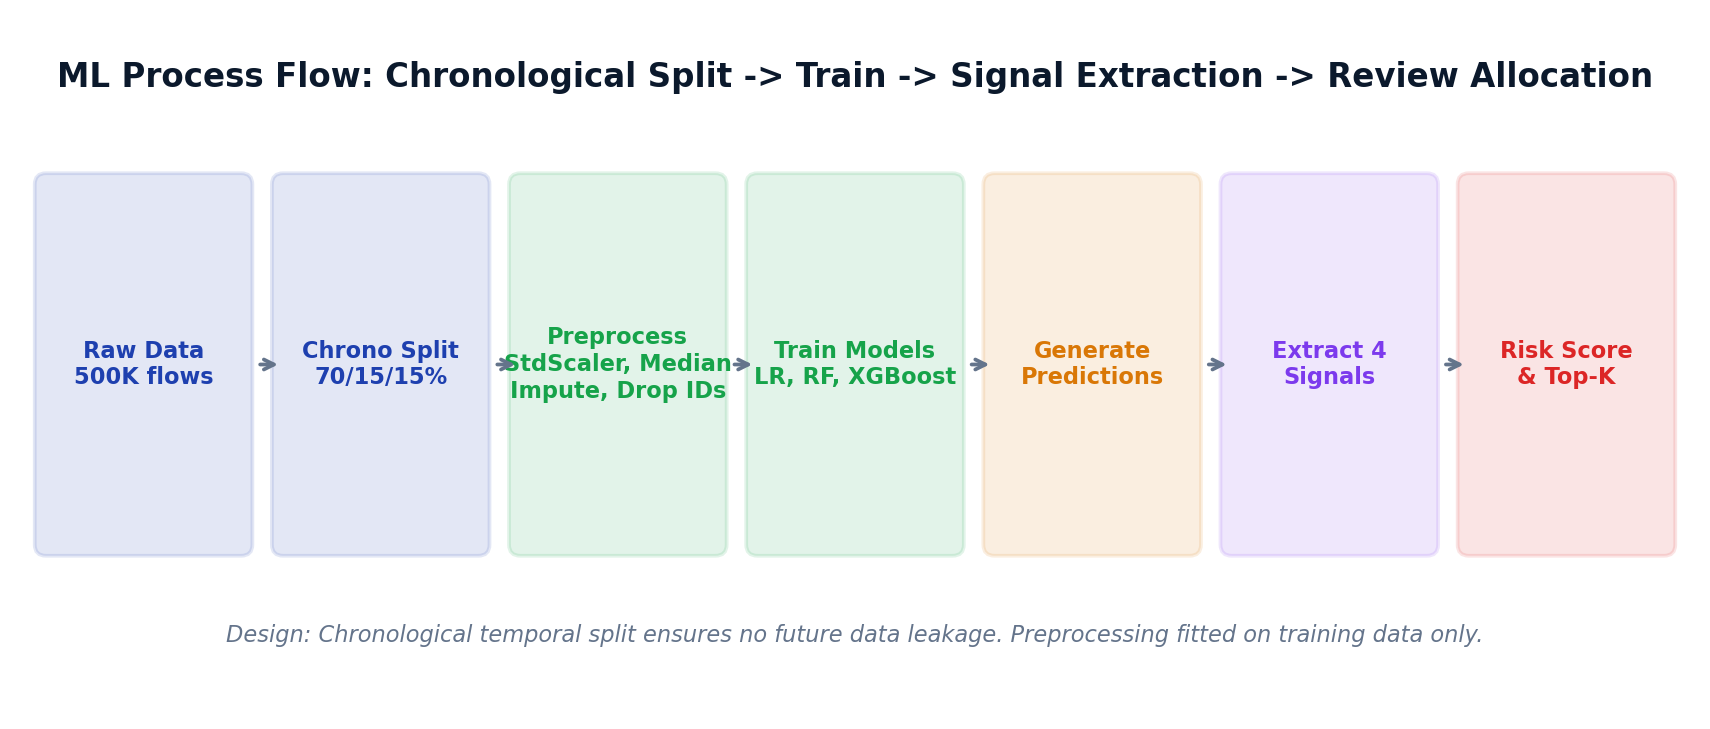
\includegraphics[width=0.85\textwidth]{figures/v2_process_flow.png}
\caption{Figure 11.3: End-to-End Operational Process Flow Diagram.}
\end{figure}

\subsection{11.5 ML / Data Processing Pipeline}

Figure 11.4 details the machine learning data processing pipeline, tracing chronological data partitioning, feature extraction, covariance matrix fitting, classifier training, and signal generation.

\begin{figure}[H]
\centering
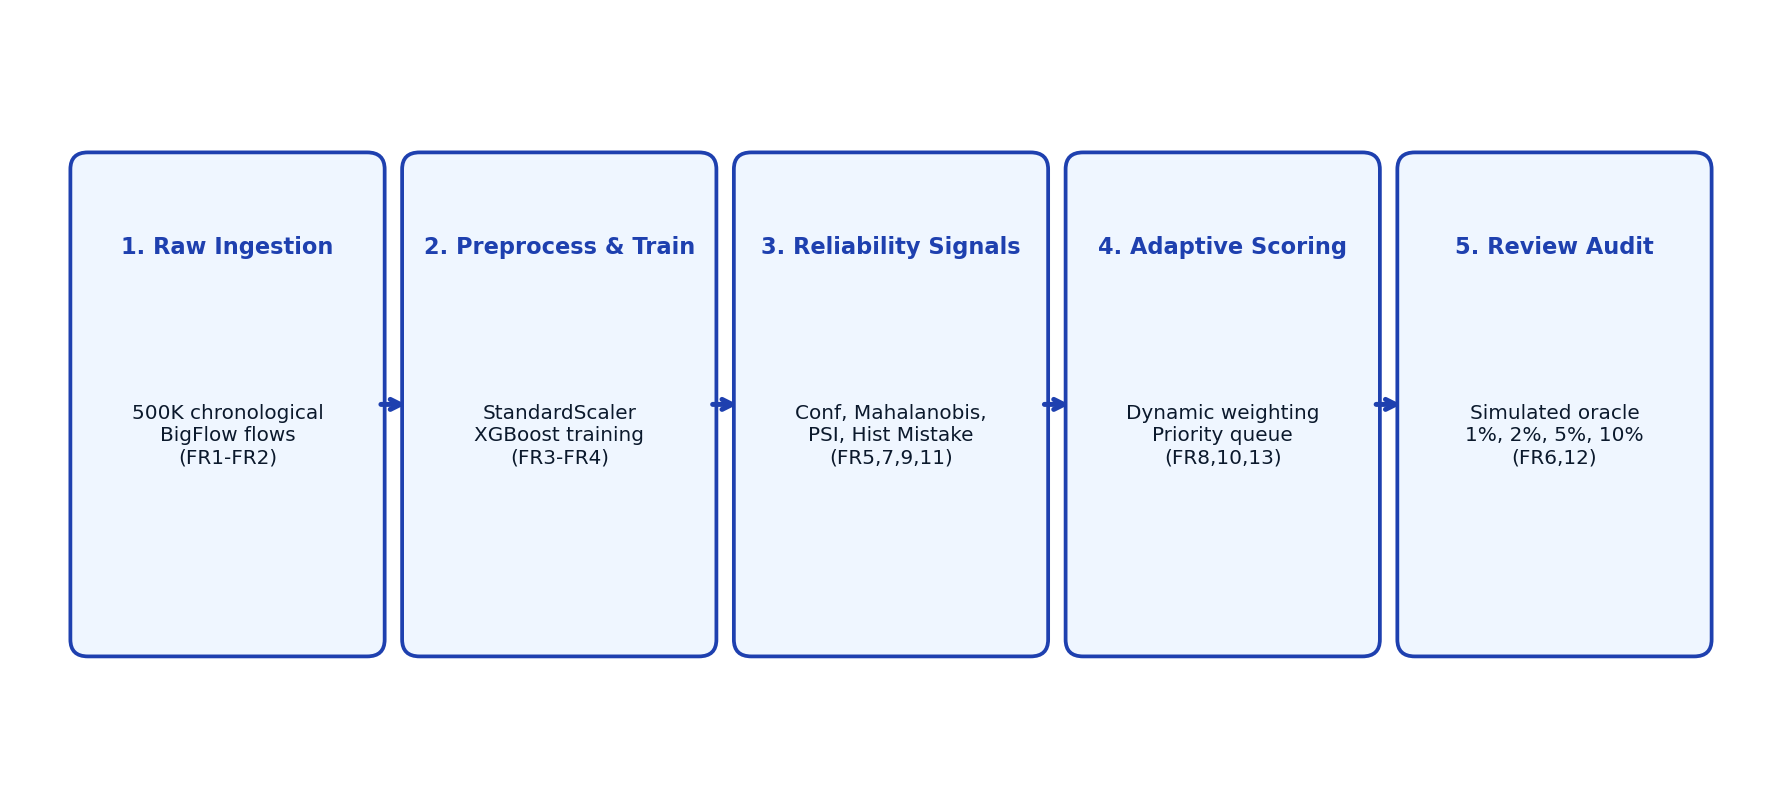
\includegraphics[width=0.85\textwidth]{figures/v2_ml_pipeline.png}
\caption{Figure 11.4: Machine Learning and Data Processing Pipeline Architecture.}
\end{figure}

\subsection{11.6 DL Model Architecture}

\textbf{Status:} Not Applicable. The project focuses on gradient boosted decision trees (XGBoost), bagging ensembles (Random Forest), and regularized linear classifiers on tabular network telemetry. Deep neural architectures were deliberately excluded because tree-based ensembles demonstrate superior empirical performance, faster inference throughput, and lower computational overhead on structured tabular cybersecurity data.

\subsection{11.7 Network / IoT Block Diagram}

\textbf{Status:} Not Applicable. The system operates as a software-based post-hoc decision layer deployed on workstation infrastructure processing tabular network flow summaries. It does not interface directly with physical IoT microcontrollers, sensor buses, or specialized embedded networking hardware.

